% Use a one-sided article template
\documentclass[oneside, 10pt]{article}
% Decrease the margins a little
\usepackage{fullpage}

% Support UTF8 input
\usepackage[utf8]{inputenc}

% Set up for including graphics
% We'll use png or pdf graphics
\usepackage[pdftex]{graphicx}
\DeclareGraphicsExtensions{.png,.pdf}

% Hyperref adds hyperlinks to the document automatically
% It's not much use yet, but it will be
\usepackage{hyperref}

% For including code into the document
\usepackage{verbatim}

% Tweak the default fonts a little
\renewcommand\rmdefault{bch}
\usepackage[small]{caption}
\usepackage[small]{titlesec}
\linespread{1.07}

% Typographic tweaks
\usepackage{microtype}
%\usepackage{}

\usepackage{subfigure}

\title{The Grammar of Graphics}
\author{Pedro Alcocer}
\date{\today}

\raggedbottom

\begin{document}
\maketitle

\noindent\texttt{ggplot2} is a plotting system for R, based on the grammar of graphics, which tries to take the good parts of the standard graphics utilities and none of the bad parts. It takes care of many of the fiddly details that make plotting a hassle (like drawing legends) as well as providing a powerful model of graphics that makes it easy to produce complex multi-layered graphics.

This module is intended to be a superficial introduction to \texttt{ggplot2}.

\section{Preliminaries}

Make certain you have installed the latest version of the packages that this document depends on with:

\begin{verbatim}
> install.packages("languageR")
> install.packages("ggplot2")
\end{verbatim}

We will be using the \texttt{english} dataset from the \texttt{languageR} package. This data set gives mean visual lexical decision latencies and word naming latencies to 2284 monomorphemic English nouns and verbs, averaged for old and young subjects, with various predictor variables.

Learn more about the \texttt{english} dataset with:

\begin{verbatim}
> ?english
\end{verbatim}

Actually inspect the dataset with:

\begin{verbatim}
> head(english)
     RTlexdec RTnaming Familiarity   Word AgeSubject WordCategory WrittenFrequency
1 6.543754 6.145044        2.37    doe      young            N         3.912023
2 6.397596 6.246882        4.43  whore      young            N         4.521789
3 6.304942 6.143756        5.60 stress      young            N         6.505784
4 6.424221 6.131878        3.87   pork      young            N         5.017280
5 6.450597 6.198479        3.93   plug      young            N         4.890349
6 6.531970 6.167726        3.27   prop      young            N         4.770685

> tail(english)
     RTlexdec RTnaming Familiarity  Word AgeSubject WordCategory WrittenFrequency
4563 6.608770 6.503839        3.70   spy        old            V         5.023881
4564 6.753998 6.446513        2.40   jag        old            V         2.079442
4565 6.711022 6.506979        3.17  hash        old            V         3.663562
4566 6.592332 6.386879        3.87  dash        old            V         5.043425
4567 6.565561 6.519884        4.97 flirt        old            V         3.135494
4568 6.667300 6.496624        3.03  hawk        old            V         4.276666
\end{verbatim}

\section{Building plots}

Suppose we are interested in discovering how the lexical decision reaction times (\texttt{RTlexdec}) are distributed. A histogram is a good way to represent a distribution. The $x$-axis should contain the reaction times and $y$-axis should contain binned counts of reaction times.

We begin a plot by describing what relationships we want to plot. The following command describes the relationship we're interested in (i.e., just the behavior of \texttt{RTlexdec}) and stores this description in the variable \texttt{p}. Calling \texttt{p} results in an empty plot window. This alone doesn't plot anything because we haven't specified the details of how to plot this abstract description.

\begin{verbatim}
> p <- ggplot(english, aes(x = RTlexdec))
> p
\end{verbatim}

\texttt{ggplot2} thinks about plots as data relationships and ways to display those relationships. Typically, the data relationships are described with the \verb!ggplot()! function. This function takes two arguments: (1) the data frame which contains your data, in this case \verb!english! and (2)  a description of the variables which you wish to plot within an \verb!aes()! function call. In this case, we are only interested in plotting something along the $x$ axis, so the call is \verb!aes(x = RTlexdec)!.

How relationships are actually plotted is handled by the \texttt{geom} and \texttt{stat} family of commands. There are many geoms available to you.\footnote{For a complete list of geom and stat commands see the online \texttt{ggplot2} reference manual at \url{http://had.co.nz/ggplot2/}} For instance, to plot a histogram, we would add the geom \verb!geom_histogram()! to the \texttt{p} object we created.

\begin{figure}[htbp]
  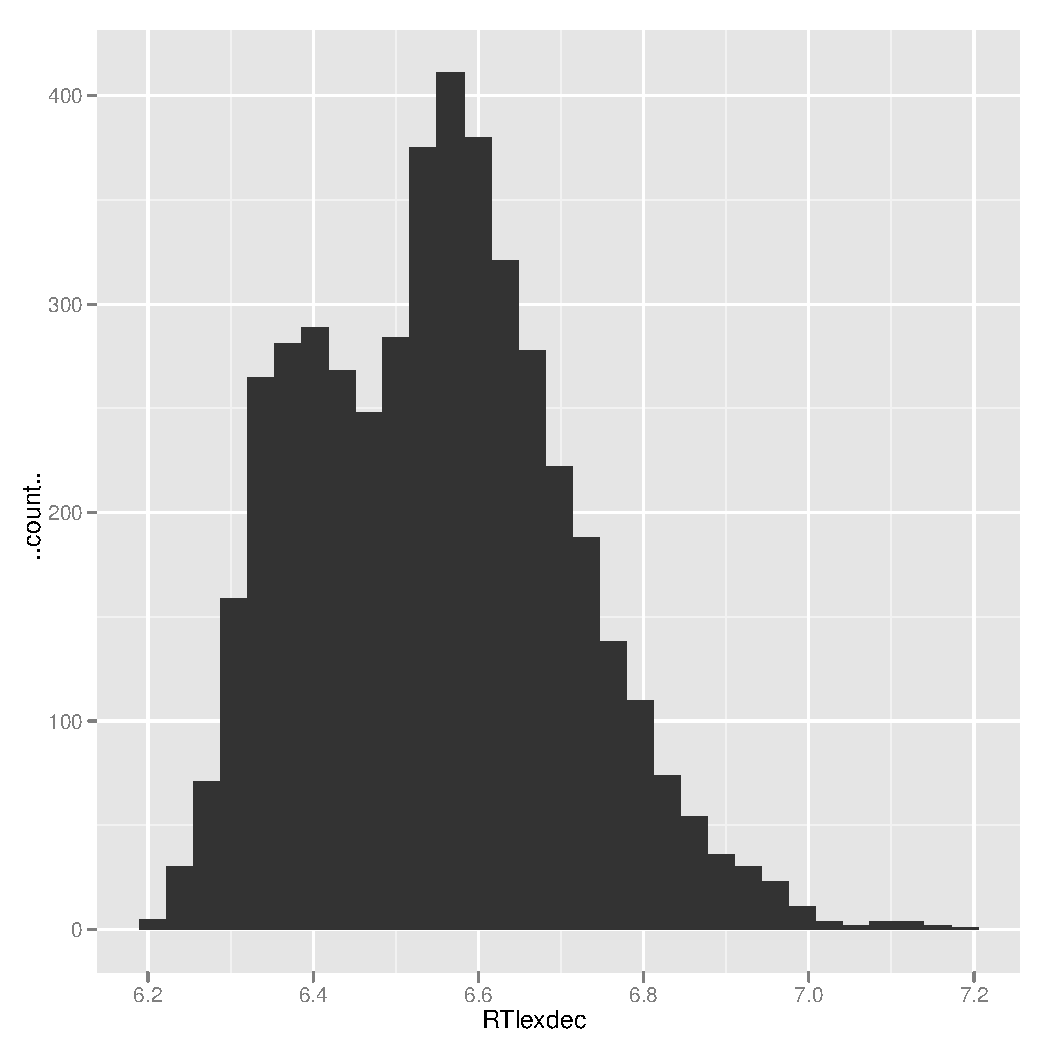
\includegraphics[width = 0.5\linewidth]{histogram}%
  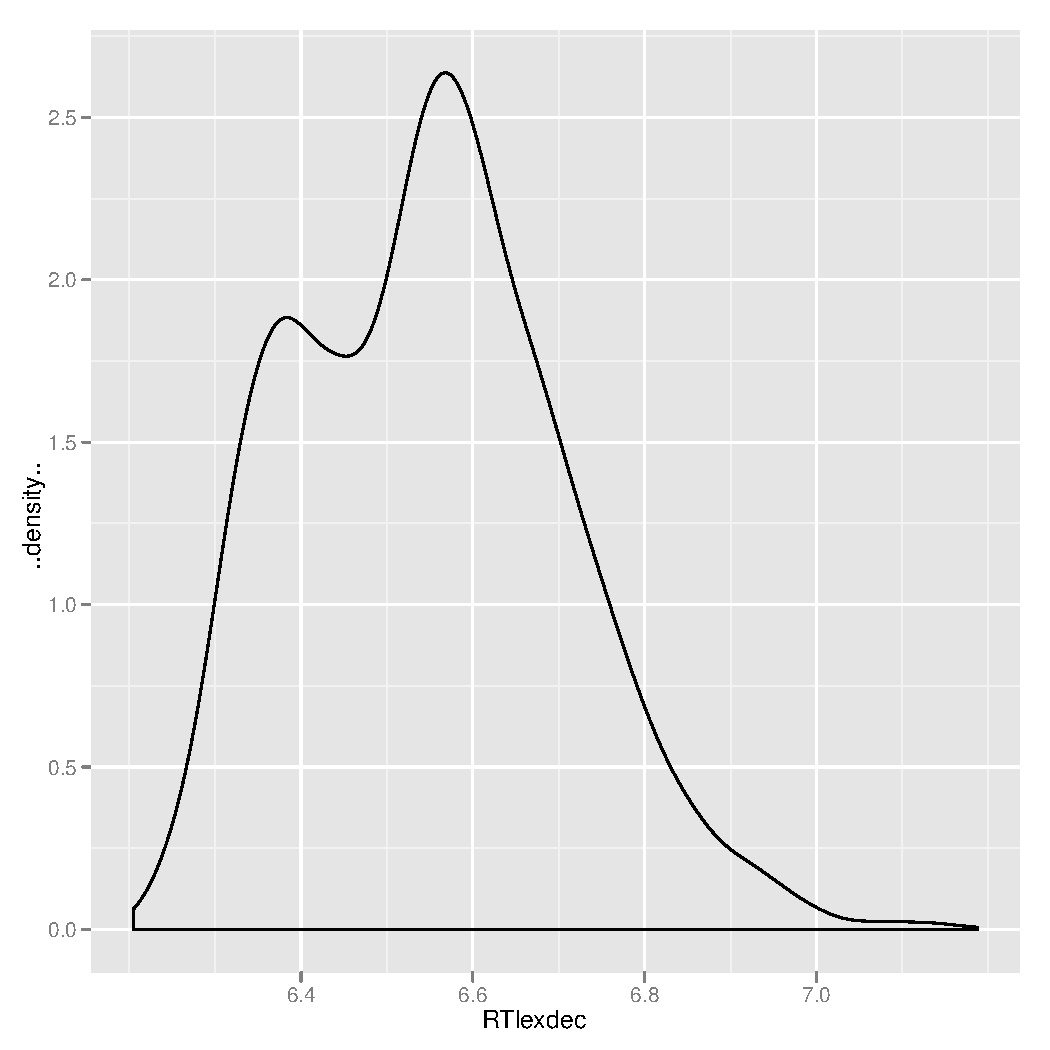
\includegraphics[width = 0.5\linewidth]{density}
  \caption{(Left) A histogram of the distribution of the \texttt{RTlexdec} response variable made with the \texttt{geom\_histogram} geom. (Right) A smooth density estimate of the same, made with the \texttt{geom\_density} geom.}
  \label{fig:one}
\end{figure}

\begin{verbatim}
> p + geom_histogram()
\end{verbatim}

To plot a smooth density estimate, we use the \texttt{geom\_density()} geom, instead.

\begin{verbatim}
> p + geom_density()
\end{verbatim}



\subsection{Plotting two variables}

Plotting two variables is similar to plotting one; it simply requires that you specify what should be plotted on the $y$ axis. Below, we set up these relationships and store the abstract plot in \verb!p2!. On the $x$ axis, we'll have the written frequency of a word (\verb!WrittenFrequency!) and on the $y$ axis we'll have the lexical decision reaction time response variable \verb!RTlexdec!.

\begin{verbatim}
> p2 <- ggplot(english, aes(x = WrittenFrequency, y = RTlexdec))
\end{verbatim}

We can now plot this relationship on a scatterplot with the \verb!geom_point()! geom.

\begin{verbatim}
> p2 + geom_point()
\end{verbatim}

Likewise, without much trouble we can make two-dimensional histograms with square or hexagonal tessellations using the \verb!geom_bin2d()! or \verb!geom_hex()! geoms.

\begin{figure}[htbp]
  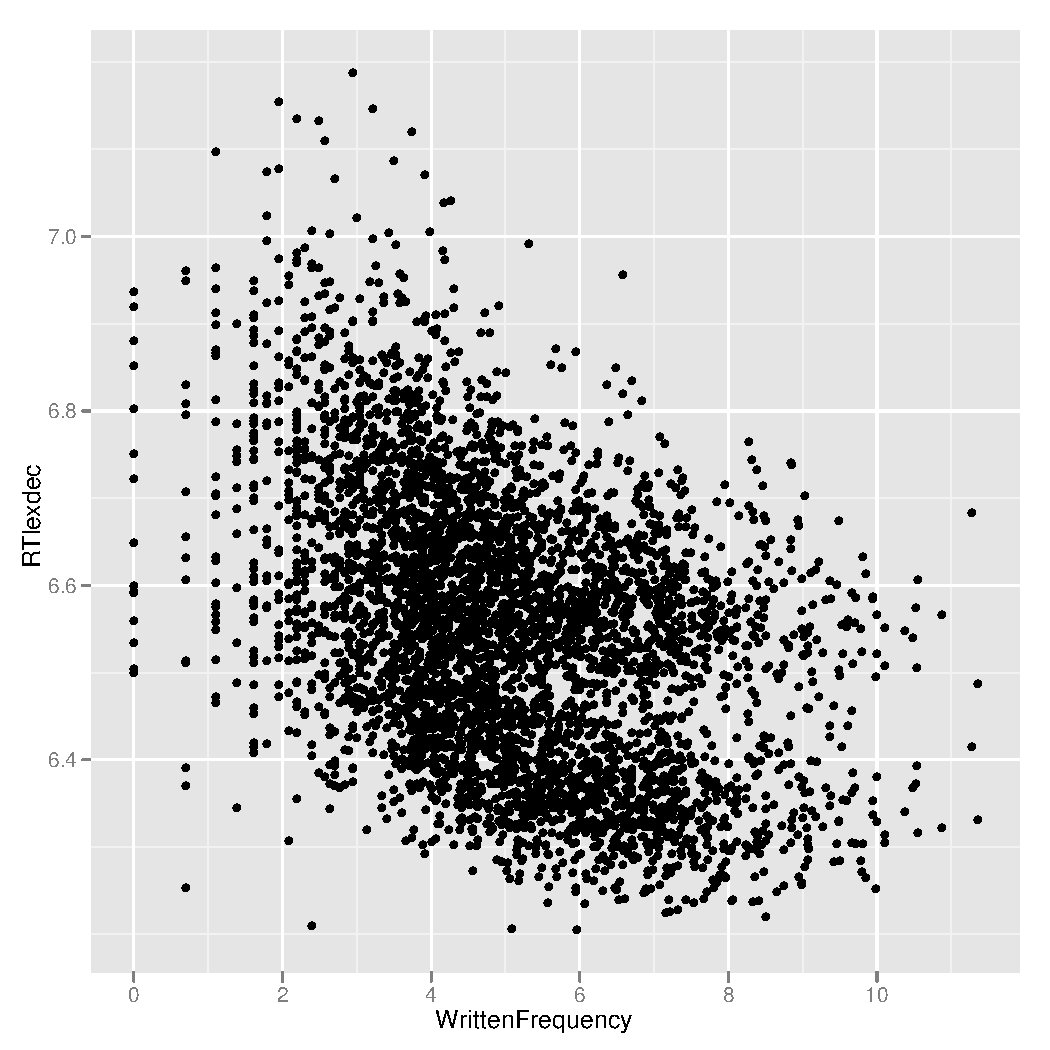
\includegraphics[width = 0.33\linewidth]{geom-point}%
  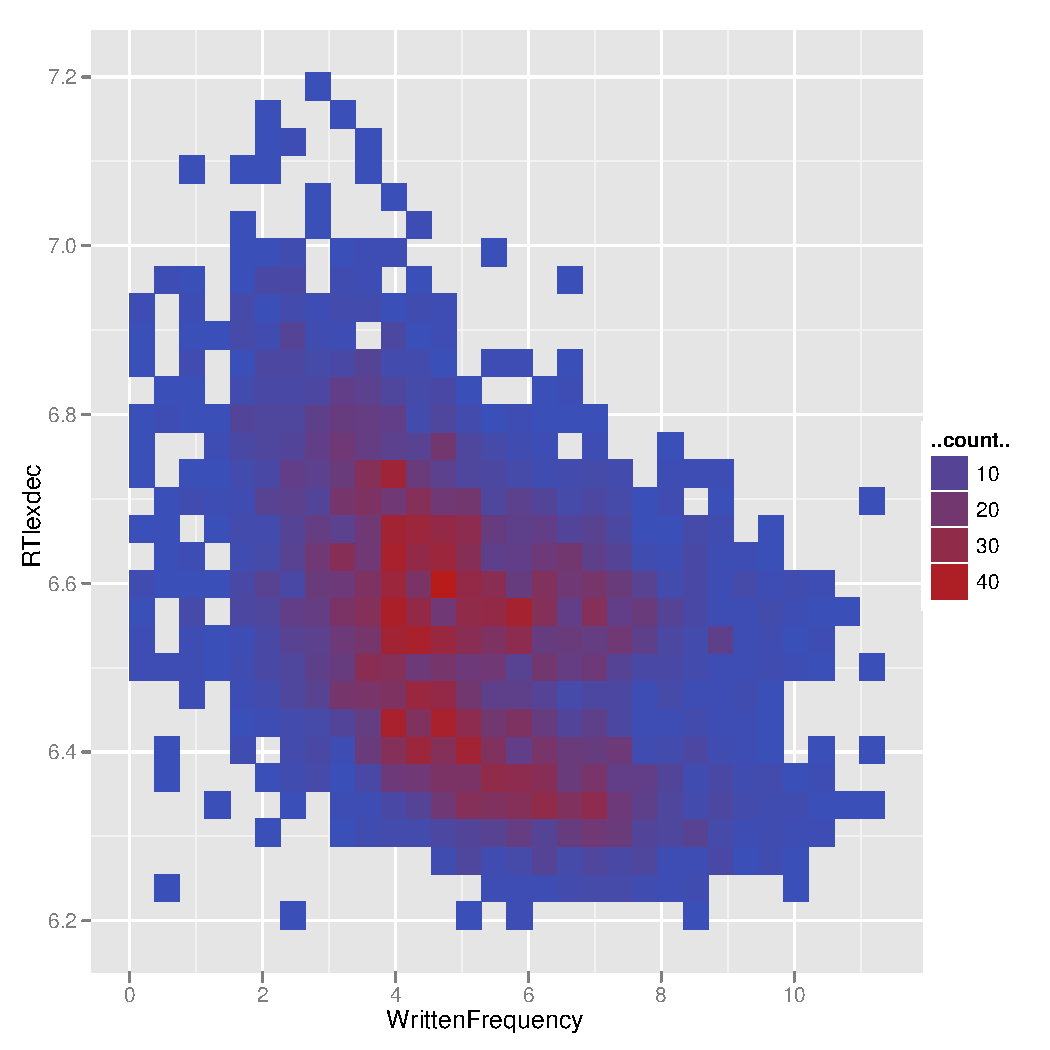
\includegraphics[width = 0.33\linewidth]{geom-bin2d}%
  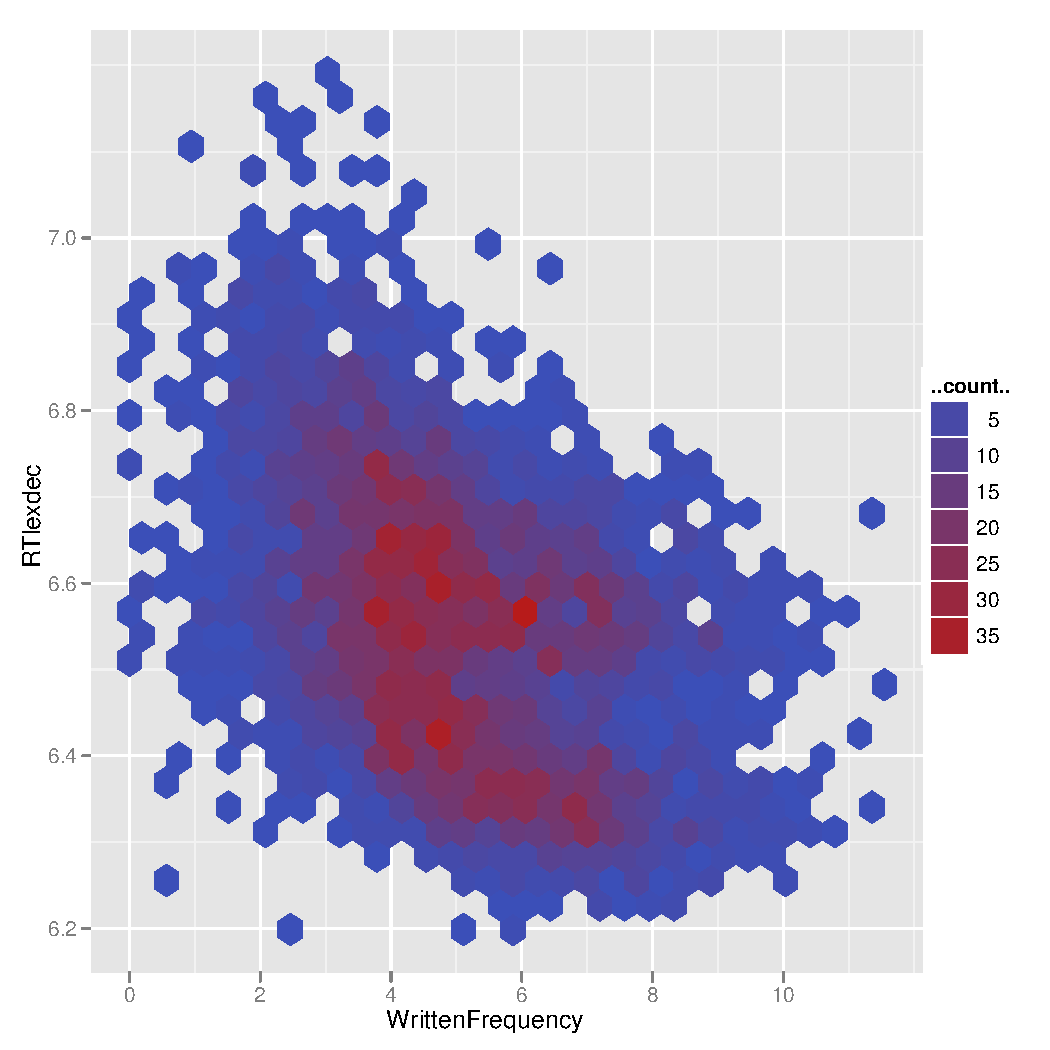
\includegraphics[width = 0.33\linewidth]{geom-hex}
  \caption{(Left) A scatter plot comparing written frequency (\texttt{WordCategory}) with log lexical decision reaction time (\texttt{RTlexdec}). (Center) A square-tessellated 2D histogram of the same relationship. (Right) A hexagon-tessellated 2D histogram.}
  \label{fig:2dplotting}
\end{figure}

So far, we haven't done much in \verb!ggplot2! that we couldn't easily do in the base R graphics system (perhaps with the exception of the 2D histograms). Let's move into some territory where \verb!ggplot2! excels.

\section{Beyond base}

Notice that the histogram and the density estimate in Figure \ref{fig:one} seem to have two peaks and that there seem to be two areas of concentration in the plots in Figure \ref{fig:2dplotting}. This may indicate that we are looking at two overlapping distributions. \verb!ggplot2! makes it very easy to split data by variable and display it in several ways.

\subsection{Splitting variables into colors}

Let's try to discover the predictor variable that is driving the two distributions. We'll consider three predictors: \verb!WordCategory!, the category of the word that is being presented, noun or verb; \verb!CV!, whether the word in question begins with a consonant or a vowel; and \verb!AgeSubject!, whether the subject falls into the ``young'' age group or the ``old'' age group. We'll plot a smoothed density estimate and separate the two levels of the factor in question. Each level will be plotted in a different color. \footnote{Notice that we are using the \texttt{aes()} command again. This command is really about \emph{aes}thetic mappings between variables in the data and the visual properties of geoms. When we pass an \texttt{aes()} call to the \texttt{ggplot()} function, we are passing those aesthetic mappings to any and all geoms that are added to that function. On the other hand, when we call \texttt{aes()} within a particular geom, the specified aesthetic mappings apply only to that geom.}

\begin{verbatim}
> p + geom_density(aes(color = WordCategory)) 
> p + geom_density(aes(color = CV))
> p + geom_density(aes(color = AgeSubject))
\end{verbatim}

\begin{figure}[htbp]
  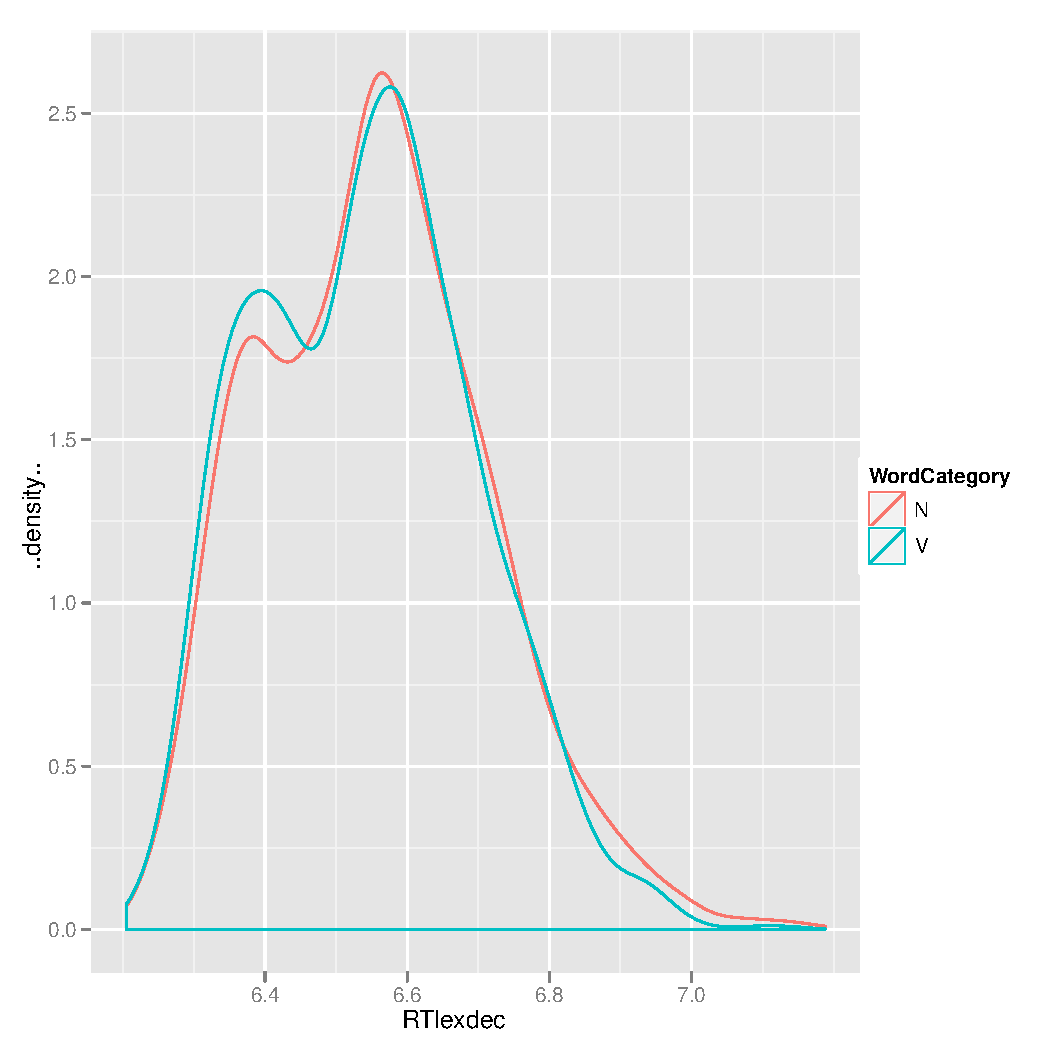
\includegraphics[width = 0.33\linewidth]{color1}%
  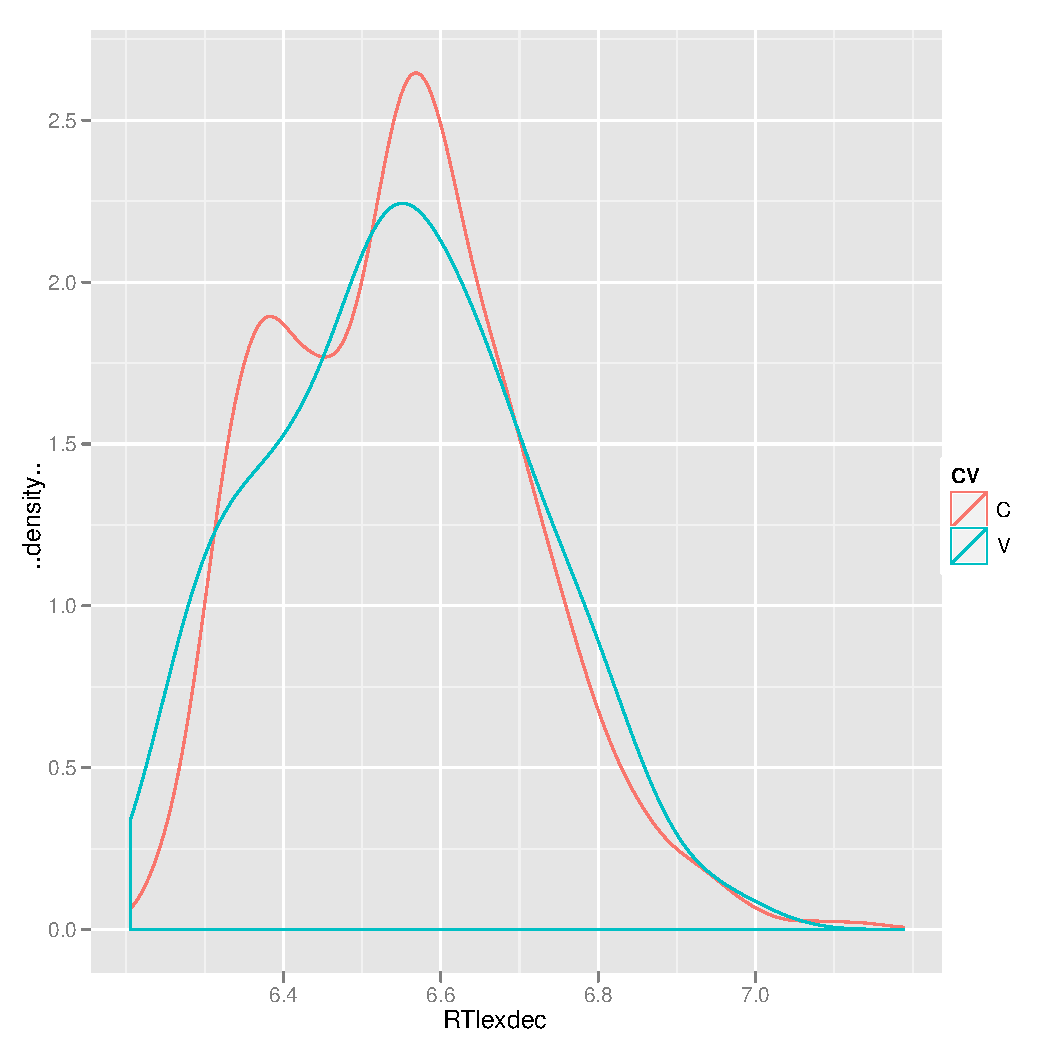
\includegraphics[width = 0.33\linewidth]{color2}%
  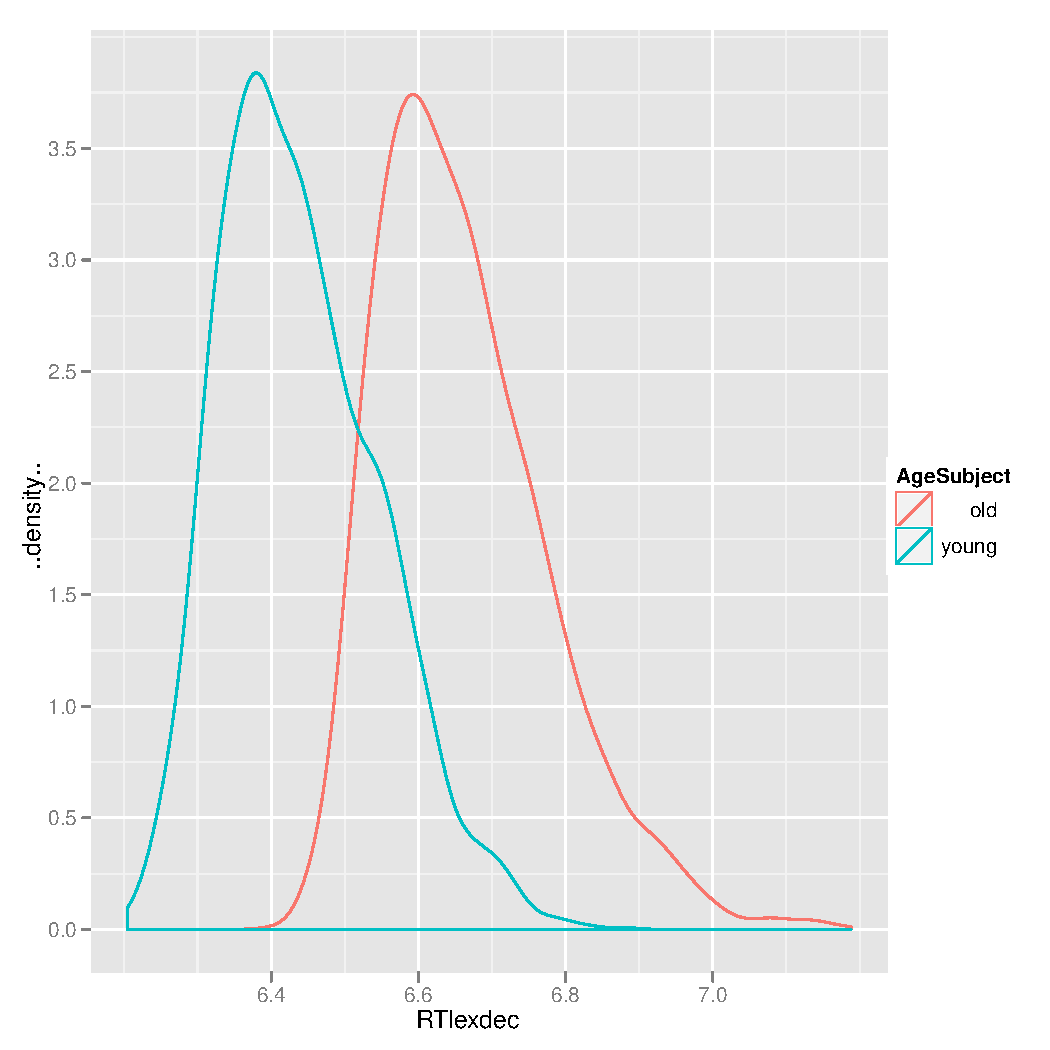
\includegraphics[width = 0.33\linewidth]{color3}%
  \caption{(Left) \texttt{WordCategory} (Center) \texttt{CV} (Right) \texttt{AgeSubject}}
  \label{fig:densities}
\end{figure}

\begin{verbatim}
> p + geom_density(aes(color = LengthInLetters)) # Doesn't work.
> p + geom_density(aes(color = factor(LengthInLetters))) # Does what you expect.
\end{verbatim}

The rightmost plot in Figure \ref{fig:densities} suggests that the two underlying distributions may be due to subject age. It seems that older subjects are slower at responding than younger subjects. We can see this again if we try a similar split on a scatterplot.

\begin{verbatim}
> p2 + geom_point(aes(color = AgeSubject))
\end{verbatim}

\begin{figure}[htbp]
  \centering
  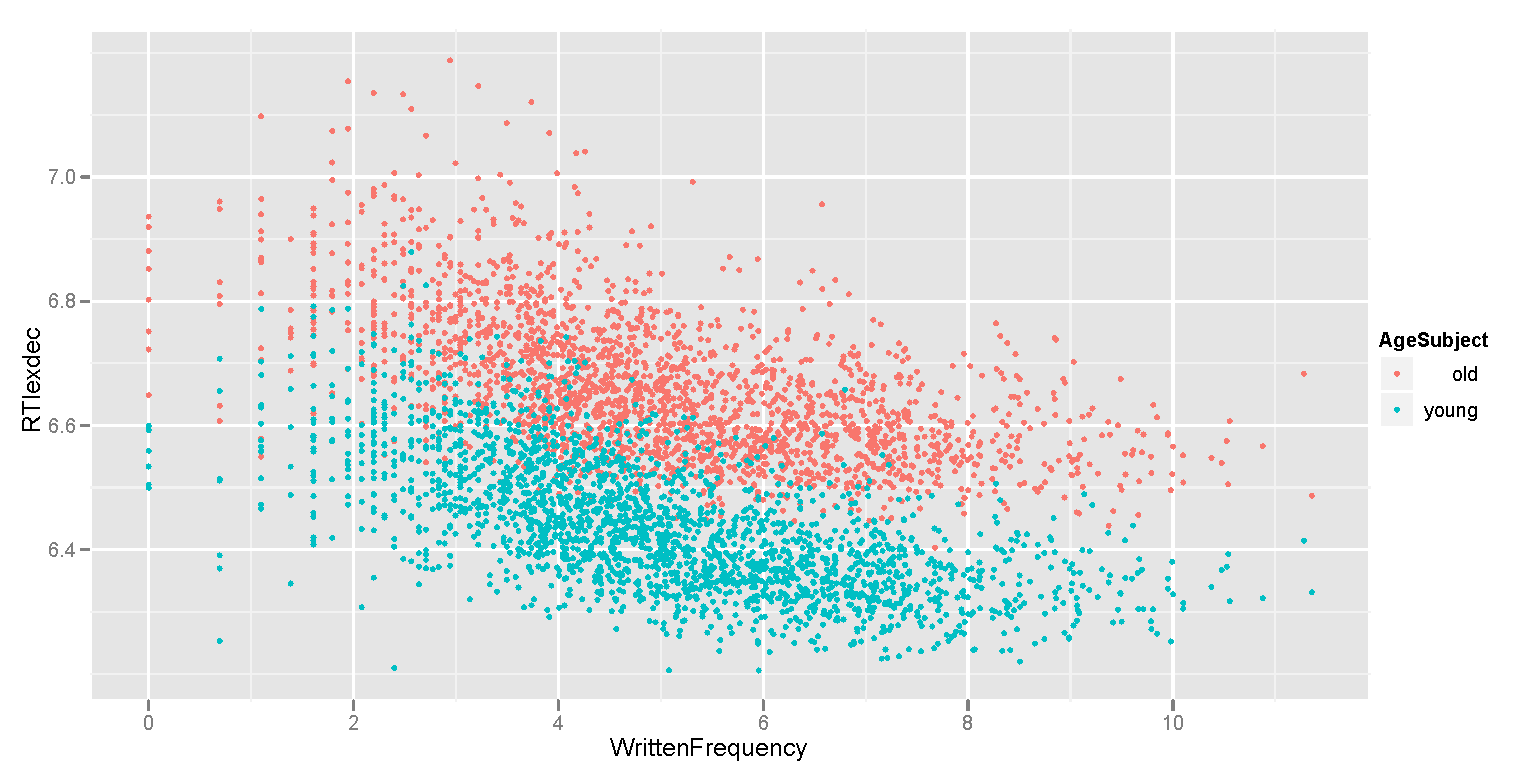
\includegraphics[width = 0.80\linewidth]{points-color}
  \caption{A scatter plot with \texttt{AgeSubject} split into different colors.}
  \label{fig:points-color}
\end{figure}

Note that the predictor variable you are splitting by must be a factor in R. You will get an error if you try to split by a numerical predictor. You can, however, convert integer predictors into factors with \verb!factor()!.

\subsection{Layering}

Part of the flexibility that \verb!ggplot2! offers is the ability to layer plots on top of each other. For instance, we can layer a 2D density contour on top of a scatter plot. In order to get a good result, I'll also be adjusting some graphical settings.

\begin{verbatim}
> % Set up a scatter plot with some transparency to prevent overplotting.
> % Note that color in this instance has nothing to do with variables, so doesn't 
> % require aes().
> scatter <- geom_point(color = alpha("black", 1/3))
>
> % Set up a 2D density contour with line thickness 1, split by AgeSubject
> % into different colors. Note that size is outside aes().
> contour <- geom_density2d(size = 1, aes(color = AgeSubject))
>
> % Apply plots to data
> p2 + scatter
> p2 + contour
> p2 + scatter + contour
\end{verbatim}

The rightmost plot in Figure \ref{fig:layers} is a useful plot because it shows the raw data---no statistical opacity here---but also allows for a transparent and striking interpretation of that data: the two distributions are clearly overlapping. Furthermore these plots were generated with a minimal amount of syntax. Here we can really see the usefulness of the \verb!ggplot2! package.

\begin{figure}[htbp]
  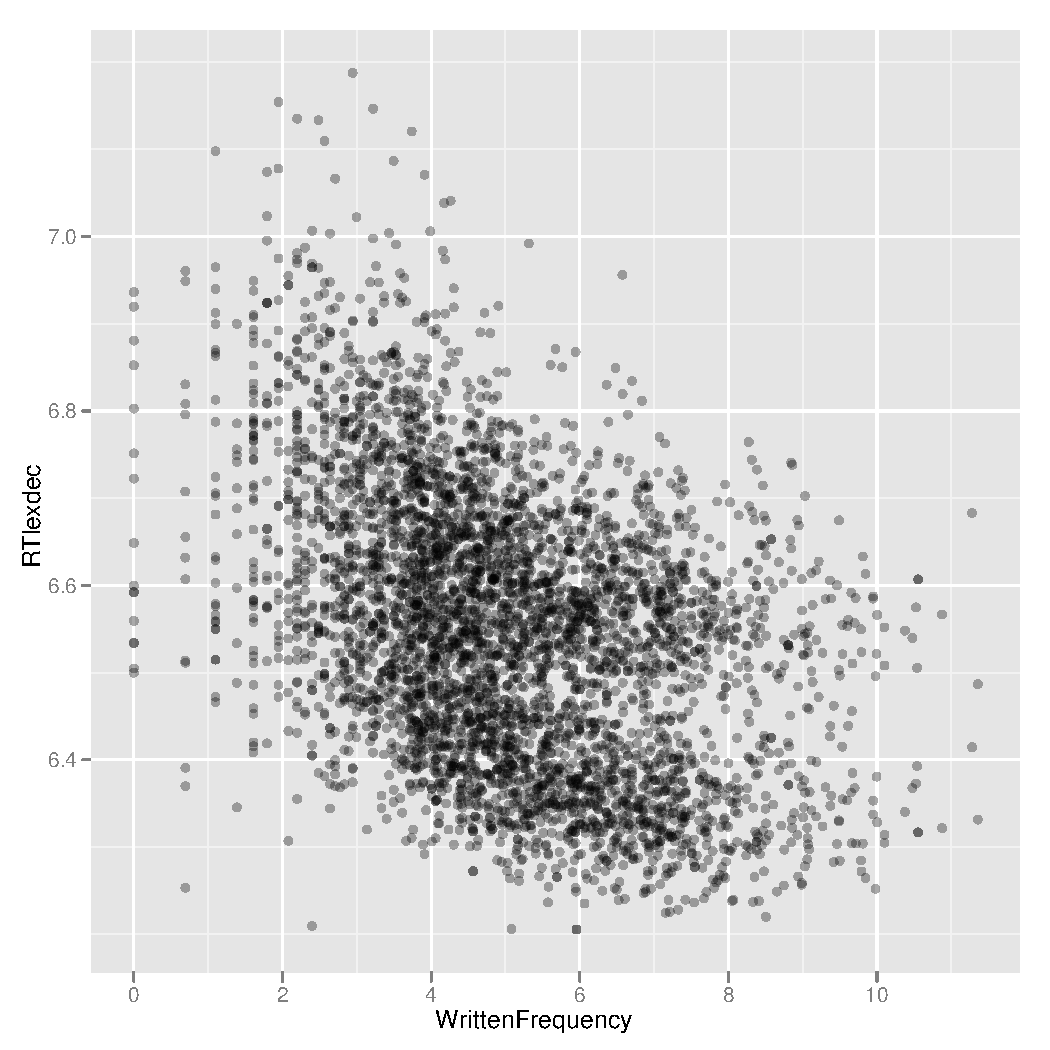
\includegraphics[width = 0.25\linewidth]{scatter}%
  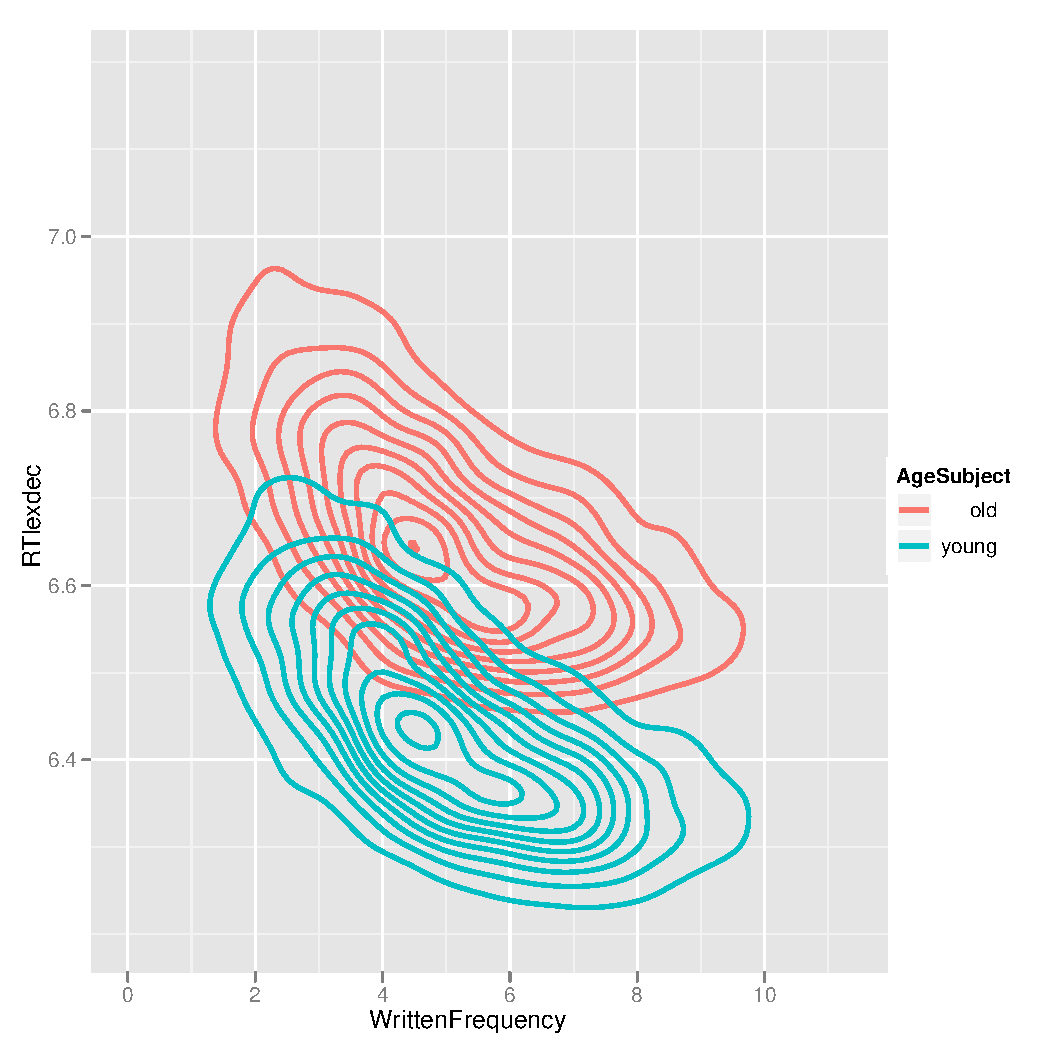
\includegraphics[width = 0.25\linewidth]{contour}%
  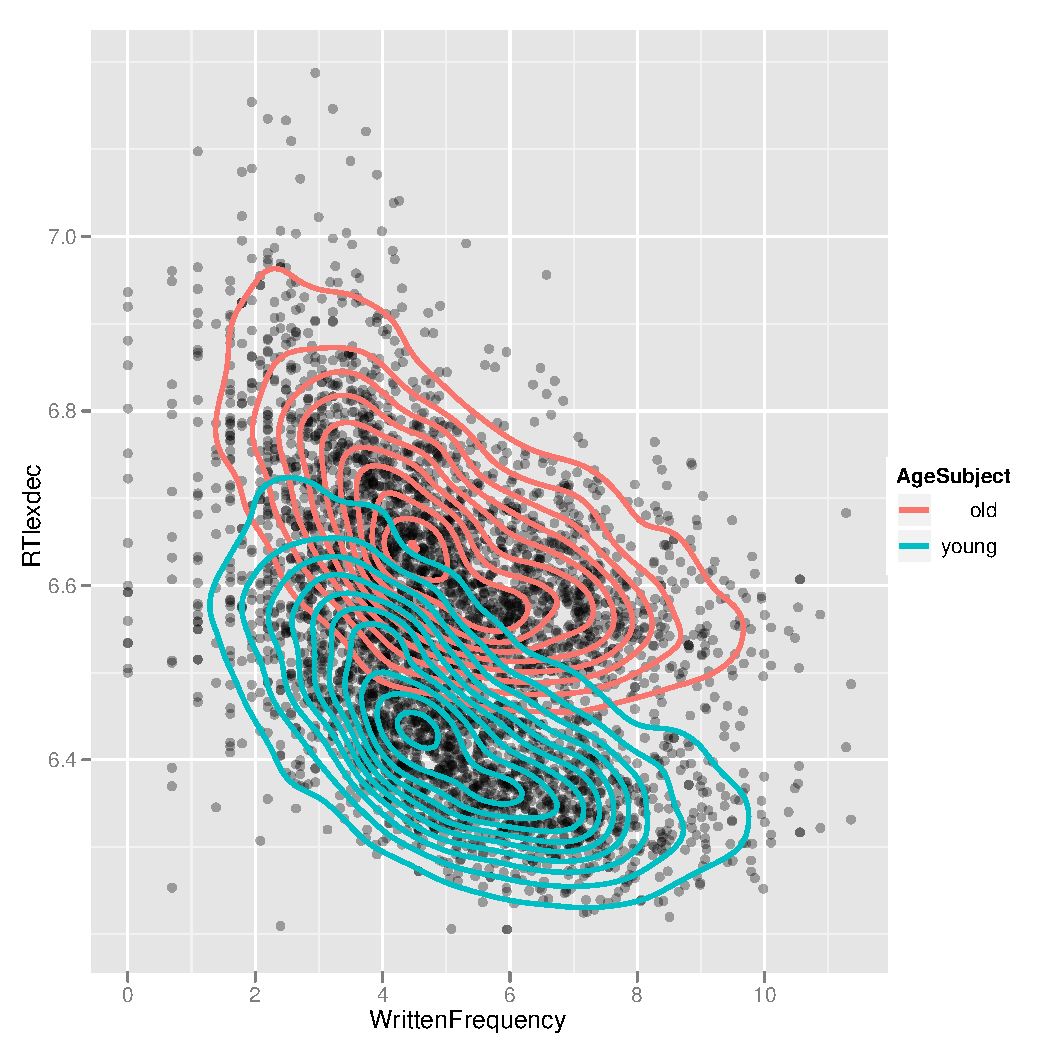
\includegraphics[width = 0.50\linewidth]{scatter-contour}%
  \caption{(Left) The first layer, a scatter plot. (Center) The second layer, a 2D density contour plot. (Right) The combined plot with raw data and contours.}
  \label{fig:layers}
\end{figure}

\subsection{Faceting}

Faceting is another way to split data on a variable. Faceting separates two levels of a factor \emph{in space}. For instance, let's facet a hexagonally-tiled 2D histogram by the \verb!AgeSubject! variable.

\begin{verbatim}
> p2 + geom_hex() + facet_grid(. ~ AgeSubject)
\end{verbatim}

\begin{figure}[htbp]
  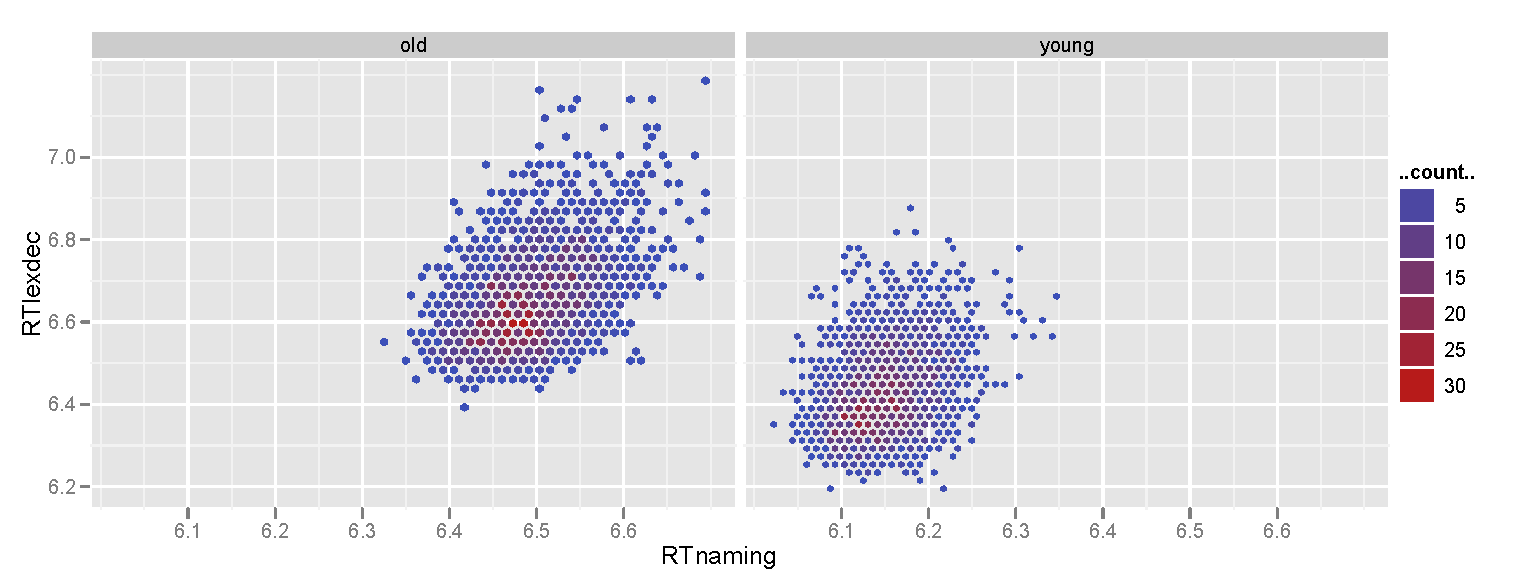
\includegraphics[width = 1\linewidth]{hexbin-facets}
  %\caption{(Left) \texttt{WordCategory} (Center) \texttt{CV} (Right) \texttt{AgeSubject}}
  \label{fig:three}
\end{figure}

\section{Stat layers}

\begin{verbatim}
> p2 + geom_point(aes(color = AgeSubject))
> p2 + geom_point(aes(color = AgeSubject)) + stat_smooth()
> p2 + geom_point(aes(color = AgeSubject)) + stat_smooth(aes(group = AgeSubject))

> p2 + geom_point(aes(color = AgeSubject))
> p2 + geom_point(aes(color = AgeSubject))
\end{verbatim}





\end{document}
